\documentclass[12pt]{beamer}
\author{Yan Wang}
\title{Paper Reading Seminar}
\subtitle{}
\usetheme{Malmoe}
\setbeamertemplate{navigation symbols}{}
\newcommand*\oldmacro{}%
\let\oldmacro\insertshorttitle%
\renewcommand*\insertshorttitle{%
\oldmacro\hfill%
\insertframenumber\,/\,\inserttotalframenumber}

\begin{document}

\begin{frame}[plain]
	\titlepage
\end{frame}

\begin{frame}{RGB-(D) Scene Labeling: Features and Algorithms}
	\begin{itemize}
		\item Problem: indoor scene, optical photo + depth image $\Rightarrow$ pixel-wise label \\
		\medskip
		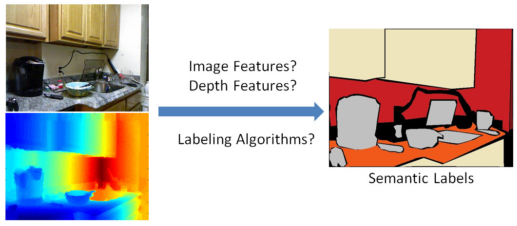
\includegraphics[width=0.5\textwidth]{fig1.png} \\
		\item Evaluation: NYU Depth Dataset (13 categories), Stanford Background Dataset (8 categories, no depth info), Mean AP.
	\end{itemize}
\end{frame}

\begin{frame}{Intuition}
	\begin{itemize}
		\item Kernel Descriptor + Efficient Matching Kernel: pixel level features in different domains $\Rightarrow$ superpixel level feature
		\item Segmentation tree: different scales of superpixel
		\item Contextual refinement
	\end{itemize}
\end{frame}

\begin{frame}{Approach}
	\begin{itemize}
		\item Segmentation trees
		\begin{itemize}
			\item gPb: local + global contrast cues $\Rightarrow$ pixel-level probability-of-boundary map
			\item Extend to depth frames
			\item Linear fusion for RGB-D frames \\
            \[\text{gPb}_\text{rgbd} = (1 - \alpha) \cdot \text{gPb}_\text{rgb} + \alpha \cdot \text{gPb}_\text{d}\]
		\end{itemize}
		\item Feature design
		\begin{itemize}
			\item Gradient, color, local binary pattern, depth gradient, spin/surface normal, KPCA/self-similarity
		\end{itemize}
	\end{itemize}
\end{frame}

\begin{frame}{Approach}
	\begin{itemize}
		\item Kernel descriptors
		\begin{itemize}
			\item Intuition: pixel features $\Rightarrow$ superpixel
			\[F_\text{grad}^t = \sum_{z\in Z}\tilde{m}_zk_o(\tilde{\theta}_z, p_i)k_s(z, q_j)\]
            ($p_i, q_j$ are randomly sampled from the superpixel)
			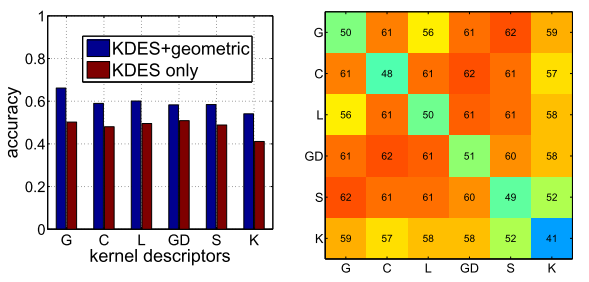
\includegraphics[width=0.7\textwidth]{fig3.png} \\
			\item Use image gradient + spin/normal
		\end{itemize}
	\end{itemize}
\end{frame}

\begin{frame}{Approach}
	\begin{columns}[l]
		\column{0.7\textwidth}
			\begin{itemize}
			\item Classification
			\begin{itemize}
				\item Efficient Match Kernel for fixed-length features on superpixels
				\item Linear SVM
				\item Normalize on superpixel area ($A_s$)
				\[A_s / (\sum_{q\in Q_c}A_q)^p\]
			\end{itemize}
			\item Segmentation tree
				\begin{itemize}
					\item Different level ($t$) of segmentation tree $\Leftrightarrow$ different scale of superpixels \\
					\item Tree(s) = $\{f_{t, c}(s_t)\}, \any t, c$
				\end{itemize}
			\end{itemize}
		\column{0.3\textwidth}
			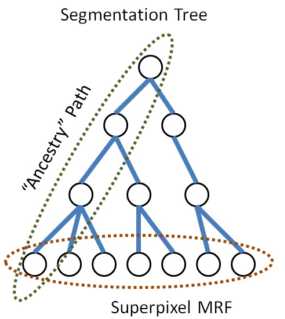
\includegraphics[width=\textwidth]{fig2.png}
	\end{columns}
\end{frame}

\begin{frame}{Approach}
	\begin{itemize}
		\item Segmentation tree
		\begin{itemize}
			\item Accumulate features along paths for better accuracy \\
			\medskip
			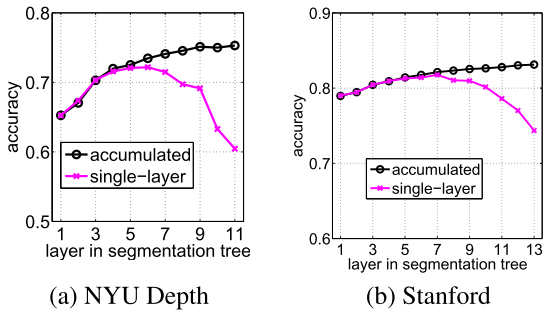
\includegraphics[width=0.5\textwidth]{fig4.png}
		\end{itemize}
		\item Superpixel MRF with gPb
		\begin{itemize}
			\item Data term: $-f_{c, t}$
			\item Smoothing term
			\[V_{s, r} = \beta \exp(-\gamma \cdot \text{gPb}_\text{rgbd}(s, r))\]
			\item Solve with graph-cut
		\end{itemize}
	\end{itemize}
\end{frame}

\end{document}
